%\documentclass{proc}  % 2-column format
\documentclass[12pt]{paper}
%\documentclass{ntmanuscript}
%\documentclass[review]{elsarticle}
\usepackage[acronym,toc]{glossaries}
\newacronym{MIT}{MIT}{the Massachusettes Institute of Technology}
\newacronym{UW}{UW}{University of Wisconsin}
\newacronym{US}{US}{United States}
\newacronym{HEU}{HEU}{highly enriched uranium}
\newacronym{LEU}{LEU}{low enriched uranium}
\newacronym{U}{U}{uranium}
\newacronym{SWU}{SWU}{separative work unit}
\newacronym{CNERG}{CNERG}{Computational Nuclear Engineering Research Group}
\newacronym{DRE}{DRE}{dynamic resource exchange}
\newacronym{UOX}{UOX}{uranium oxide}
\newacronym{MOX}{MOX}{mixed oxide}


\newacronym{IAEA}{IAEA}{International Atomic Energy Agency}
\newacronym{SNF}{SNF}{spent nuclear fuel}
\newacronym{HLW}{HLW}{high level waste}
\newacronym{FEHM}{FEHM}{Finite Element Heat and Mass Transfer}
\newacronym{DOE}{DOE}{Department of Energy}
\newacronym{GENIUSv1}{GENIUS}{Global Evaluation of Nuclear Infrastructure 
Utilization Scenarios, Version 1}
\newacronym{GENIUSv2}{GENIUS}{Global Evaluation of Nuclear Infrastructure Utilization Scenarios, Version 2}
\newacronym{GDSM}{GDSM}{Generic Disposal System Model}
\newacronym{GDSE}{GDSE}{Generic Disposal Sytem Environment}
\newacronym{GPAM}{GPAM}{Generic Performance Asessment Model}
\newacronym{FEPs}{FEPs}{Features, Events, and Processes}
\newacronym{EBS}{EBS}{Engineered Barrier System}
\newacronym{EDZ}{EDZ}{Excavation Disturbed Zone}
\newacronym{YMR}{YMR}{Yucca Mountain Repository Site}
\newacronym{EPA}{EPA}{Environmental Protection Agency}
\newacronym{PEI}{PEI}{Peak Environmental Impact}
\newacronym{VISION}{VISION}{the Verifiable Fuel Cycle Simulation Model}
\newacronym{NUWASTE}{NUWASTE}{Nuclear Waste Assessment System for Technical Evaluation}
\newacronym{NWTRB}{NWTRB}{Nuclear Waste Technical Review Board}
\newacronym{OCRWM}{OCRWM}{Office of Civillian Radioactive Waste Management}
\newacronym{UFD}{UFD}{Used Fuel Disposition}
\newacronym{DYMOND}{DYMOND}{Dynamic Model of Nuclear Development }
\newacronym{DANESS}{DANESS}{Dynamic Analysis of Nuclear Energy System Strategies}
\newacronym{CAFCA}{CAFCA}{ Code for Advanced Fuel Cycles Assessment }
\newacronym{ORION}{ORION}{O..}
\newacronym{NFCSim}{NFCSim}{Nuclear Fuel Cycle Simulator}
\newacronym{COSI}{COSI}{Commelini-Sicard}
\newacronym{FCT}{FCT}{Fuel Cycle Technology}
\newacronym{SWF}{SWF}{Separations and Waste Forms}
\newacronym{FCO}{FCO}{Fuel Cycle Options}
\newacronym{RDD}{RD\&D}{Research Development and Design}
\newacronym{WIPP}{WIPP}{Waste Isolation Pilot Plant}
\newacronym{ANDRA}{ANDRA}{Agence Nationale pour la gestion des D\'echets RAdioactifs, the French National Agency for Radioactive Waste Management}
\newacronym{TSM}{TSM}{Total System Model}
\newacronym{LANL}{LANL}{Los Alamos National Laboratory}
\newacronym{INL}{INL}{Idaho National Laboratory}
\newacronym{ANL}{ANL}{Argonne National Laboratory}
\newacronym{SNL}{SNL}{Sandia National Laboratory}
\newacronym{LBNL}{LBNL}{Lawrence Berkeley National Laboratory}
\newacronym{LLNL}{LLNL}{Lawrence Livermore National Laboratory}
\newacronym{NAGRA}{NAGRA}{National Cooperative for the Disposal of Radioactive Waste}
\newacronym{CUBIT}{CUBIT}{CUBIT Geometry and Mesh Generation Toolkit}
\newacronym{CSNF}{CSNF}{Commercial Spent Nuclear Fuel}
\newacronym{DSNF}{DSNF}{DOE Spent Nuclear Fuel}
\newacronym{MTHM}{MTHM}{Metric Ton of Heavy Metal}
\newacronym{HTGR}{HTGR}{High Temperature Gas Reactor}
\newacronym{TRISO}{TRISO}{Tristructural Isotropic}
\newacronym{MA}{MA}{Minor Actinide}
\newacronym{CEA}{CEA}{Commissariat a l'Energie Atomique et aux Energies Alternatives}
\newacronym{SKB}{SKB}{Svensk Karnbranslehantering AB}
\newacronym{SINDAG}{SINDA{\textbackslash}G}{Systems Improved Numerical Differencing Analyzer $\backslash$ Gaski}
\newacronym{STC}{STC}{Specific Temperature Change}
\newacronym{LDRD}{LDRD}{Laboratory Directed Research and Development}
\newacronym{LCOE}{LCOE}{Levelized Cost of Electricity}
\newacronym{ABM}{ABM}{Agent-Based Modeling}
\newacronym{COTS}{COTS}{Commercial, Off-The-Shelf}
\newacronym{API}{API}{Application Programming Interface}
\newacronym{RIF}{RIF}{Region-Institution-Facility}
\newacronym{GUI}{GUI}{Graphical User Interface}
\newacronym{HPC}{HPC}{High-Performace Computing}
\newacronym{HTC}{HTC}{High-Throughput Computing}
\newacronym{UML}{UML}{Unified Modeling Language}
\newacronym{DAG}{DAG}{Directed Acyclic Graph}
\newacronym{XML}{XML}{Extensible Markup Language}
\newacronym{RNG}{RelaxNG}{REgular LAnguage for XML Next Generation}
\newacronym{JSON}{JSON}{JavaScript Object Notation}
\newacronym{SQL}{SQL}{Structured Query Language}
\newacronym{SQLite}{SQLite}{Structured Query Lite}
\newacronym{HDF5}{HDF5}{Hierarchical Data Format version 5}
\newacronym{CSV}{CSV}{Comma-Separated Value}
\newacronym{VL}{VL}{Variable Length}
\newacronym{SHA1}{SHA1}{Secure Hash Algorithm 1}
\newacronym{YAML}{YAML}{Yet-Another Markup Language}
\newacronym{POSIX}{POSIX}{Portable Operating System Interface}
%\newacronym{<++>}{<++>}{<++>}
%\newacronym{<++>}{<++>}{<++>}
%\newacronym{<++>}{<++>}{<++>}
%\newacronym{<++>}{<++>}{<++>}

%\makeglossaries
%%%%%%%%%%%%%%%%%%%%%%%%%%%%%%%%%%%

\usepackage{color}
\usepackage{graphicx}
\usepackage{booktabs} % nice rules for tables
\usepackage{microtype} % if using PDF
\usepackage{xspace}
\usepackage{listings}
\usepackage{textcomp}
\usepackage{ulem}

% Page length commands go here in the preamble
\setlength{\oddsidemargin}{-0.25in} % Left margin of 1 in + 0 in = 1 in
\setlength{\textwidth}{7in}   % Right margin of 8.5 in - 1 in - 6.5 in = 1 in
\setlength{\topmargin}{-.75in}  % Top margin of 2 in -0.75 in = 1 in
\setlength{\textheight}{9.2in}  % Lower margin of 11 in - 9 in - 1 in = 1 in


\definecolor{listinggray}{gray}{0.9}
\definecolor{lbcolor}{rgb}{0.9,0.9,0.9}
\lstset{
    %backgroundcolor=\color{lbcolor},
    language={C++},
    tabsize=4,
    rulecolor=\color{black},
    upquote=true,
    aboveskip={1.5\baselineskip},
    belowskip={1.5\baselineskip},
    columns=fixed,
    extendedchars=true,
    breaklines=true,
    prebreak=\raisebox{0ex}[0ex][0ex]{\ensuremath{\hookleftarrow}},
    frame=single,
    showtabs=false,
    showspaces=false,
    showstringspaces=false,
    basicstyle=\scriptsize\ttfamily\color{green!40!black},
    keywordstyle=\color[rgb]{0,0,1.0},
    commentstyle=\color[rgb]{0.133,0.545,0.133},
    stringstyle=\color[rgb]{0.627,0.126,0.941},
    numberstyle=\color[rgb]{0,1,0},
    identifierstyle=\color{black},
    captionpos=t,
}

\newcommand{\code}[1]{\lstinline[basicstyle=\ttfamily\color{green!40!black}]|#1|}
\newcommand{\units}[1] {\:\text{#1}}%
\newcommand{\SN}{S$_N$}
\newcommand{\cyclus}{\textsc{Cyclus}\xspace}
\newcommand{\Cyclus}{\cyclus}
\newcommand{\citeme}{\textcolor{red}{CITE}\xspace}
\newcommand{\TODO}[1] {{\color{red}\textbf{TODO: #1}}}%

\newcommand{\comment}[1]{{\color{green}\textbf{#1}}}

%%%%%%%%%%%%%%%%%%%%%%%%%%%%%%%%%%%
\begin{document}


%\begin{frontmatter}
\title{Modeling Material Diversion with the Cyclus Nuclear Fuel Cycle Simulator
}

% Authors. Separated by commas
\author{
  Meghan B. McGarry$^1$,
  Chris Hoffman$^1$,
  Drew Buys$^1$,
  Baptiste Mouginot$^1$,
  Paul P.H. Wilson$^1$}


\date{}
% Institutes of the authors
\institution{$^1$Department of Nuclear Engineering and Engineering Physics,
University of Wisconsin-Madison}
%\\$^2$Sandia National Laboratories}
% Information concerning the person submitting the manuscript
%\submitter{Meghan B. McGarry}
%\submitteraddress{1500 Engineering Drive, Madison, WI, USA}
%\submitteremail{mbmcgarry@wisc.edu}

% No more than three keywords, though each can be a phrase
%\keywords{fuel cycle, simulatiom, non-proliferation}
\maketitle



\begin{abstract}

  Already the dominant source of clean energy, nuclear power is growing at a
  rapid pace.  While beneficial to a world confronting climate change, there
  are increasingly serious nuclear security and non-proliferation concerns
  attendant to expanding nuclear power. As a result, it is imperative to develop
  credible methods to verify compliance with treaties that control fissile
  material production, such as the \gls{NPT} or a potential
  \gls{FMCT}. As part of the Consortium for Verification
  Technology, the Cyclus fuel cycle simulator is being used to model current
  and next-generation nuclear fuel cycles and inform treaty verification. Cyclus
  is an agent-based, systems-level simulator that tracks discrete material flow
  through the entire fuel cycle, from mining through burnup in reactors to a
  repository, or alternatively through one or more iterations of reprocessing.
  Cyclus includes social-behavior models of individual actors, facilitating the
  study of clandestine material diversion from declared fuel cycles.  Cyclus
  also features a region-institution-facility hierarchy that can incorporate the
  effects of tariffs and sanctions in a regional or global context.  This paper
  presents initial Cyclus simulations of highly enriched uranium diversion from
  a declared once-through fuel cycle.  Simulated material flow signals are
  analyzed to look for potential diversion of nuclear material for nuclear
  weaponry uses.


\end{abstract}


%\end{frontmatter}


\section{Motivation}
\label{s_motive}

In the 70 years since nuclear bombs were dropped on Hiroshima and Nagasaki, the knowledge and technology required to make these weapons has proliferated around the globe. There are now nine states that have developed their own nuclear weapons, as well as many others who have the capability to do so\cite{feiveson_unmaking_2014}.  Moreover, this knowledge will continue to spread as climate change change further tilts the scales such that the benefits of nuclear power outweigh the risks \cite{mooney_why_2014}.  China is already investing heavily in nuclear power, planning to triple its generating capacity from 19GWe to 58GWe by 2020  \cite{_china_2014}.  As climate change increasingly dominates discussions of national security, the perception of the risks inherent to nuclear energy is decreasing and states are embracing nuclear energy as a reliable large-scale source of carbon-neutral energy.  However, the expansion of nuclear power increases concerns with respect to nuclear security, because the same technologies used to produce nuclear fuel can also be exploited in the pursuit of nuclear weapons.


\subsection{Sensitive Parts of the Nuclear Fuel Cycle}

Two nuclear technologies are of of particular concern for proliferation, uranium enrichment and plutonium reprocessing.  Urnaium enrichment is required for the once-through fuel cycles that are dominant around the world today, and used exclusively in the US.  A once-through fuel cycle includes a source of natural uranium such as a mine, and is comprised of non-fissile 99.3\% $^{238}U$ and only 0.7\% fissile $^{235}U$. Concentrations of 4-20\% fissile $^{235}U$ are required to fuel a nuclear reactor. Enrichment facilities are used to increase the concentration of $^{235}U$ to the desired amount.  Fuel is then burned in a nuclear reactor and the remaining material, which includes the original $^{238}U$, short- and long-lived fission products, as well as \~1\% $^{239}Pu$ and $^{240}Pu$, is then stored as waste.  The enrichment facility is notable because it can be used to increase the concentration of $^{235}U$ up to the 80-90\% required to make a nuclear weapon\cite{_military_2014}.

Several countries are developing nuclear reactors that can accomodate recycled fuel \cite{_processing_2015}.  Recycled fuel is plutonium-based rather than uranium-based, and is made by separating the components of spent uranium fuel and increasing the concentration of fissile $^{239}Pu$ up to 80\%.  This material can then be used as fuel or blended with uranium to make \gls{MOX}.  As with the enrichment process however, separations facilities can increase the concentration beyone that required for fuel to generate \gls{WGP} (up to 93\% $^{239}Pu$).  However, fuel cycles with the capability to burn \gls{MOX} fuel are advangteous because \gls{WGP} from decommissioned nuclear weapons can be blended into \gls{MOX}, which reduces the amount of \gls{SNM} that must be safeguarded.  In part due to the large stockpile of \gls{WGP} in the \gls{US}, reprocessessing has been considered at several times over the past half-century.  However, a host of political, economic, environmental and strategic concerns have cpushed the issue of reprocessing out of the technical realm and it has become a contentious political topic, and currently the \gls{US} is pursuing only basic science research in this field \cite{rossin_policy_????, _adieu_2009}.
 
\subsection{Use of Treaties to Minimize Proliferation}

While it has not proven possible to prevent the spread of nuclear knowledge entirely, international treaties have been used in an attempt to control it.  The \gls{NPT}, which has been signed by 190 states including the original 5 nuclear weapons states, has codified a set of rules and norms for allowing the peaceful pursuit of nuclear energy\cite{_treaty_????}.  The \gls{NPT} created an organization called \gls{IAEA}, whose role is to verify compliance with the treaty by periodically inspecting facilities related to nuclear technology.  Other notable treaties include \gls{CTBT}, which placed a moratorium on testing nuclear weapons, and the \gls{START} in which the \gls{US} and Russia agreed on nuclear arms reductions.

These treaties seek to have done much to prevent the spread of nuclear weapons, but they do not address the production capabilities of states that already posess nuclear weapons.  A potential \gls{FMCT} would place limits on the amount of \gls{SNM} each weapons state could stockpile, possibly including current stockpiles in addition to future production.  However, a major unresolved issue is the difficulty of developing verification techniques that can reliably confirm that nuclear material is not being produced \cite{_fissile_2013}.  Furthermore, making measurements of nuclear material for treaty verification is itself a sensitive issue, as even collecting the spectra of a material to confirm its authenticity can potentially expose sensitive information\cite{glaser_zero_2014}. Particularly if non-weapons states are to contribute to treaty verification, it is important to prevent the further dissemination of nuclear knowledge.

\begin{figure}%[htbp!]
\begin{center}
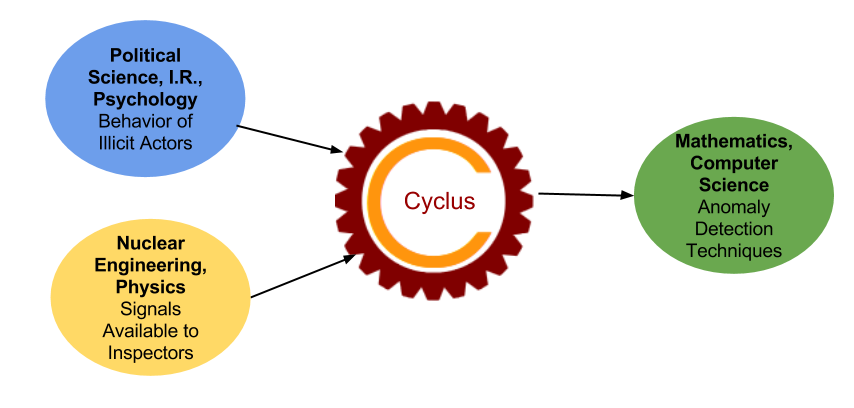
\includegraphics[natwidth=162bp,natheight=227bp, scale=0.5]{./figs/cyclus_interdiscipline.png}
\end{center}
\caption{The \Cyclus nuclear fuel cycle simulator provides a testbed to integrate innovations in treaty verification across many disciplines.}
\label{fig:cyclus_diagram}
\end{figure}

An effective treaty verification regime must synthesize knowledge from the realmns of political science, international relations, nuclear physics and engineering, and even behavioral psychology.  A nuclear fuel cycle simulator provides a framework in which to integrate these disparate components into an effective strategy.  As shown in Figure \ref{fig:cyclus_diagram}, a fuel cycle simulator can combine the technical specifications of innovative detection modalities, signal processing techniques, and models of the social-behavioral interactions between actors to provide insights into proposed verification approaches.  At a systems level, a fuel cycle simulator can be used to frame test scenarios as responses to stimuli. That is, even if not all of the specific details are available, simulations can incorporate response behaviors to illucidate the strengths and weaknesses of various verification strategies.



\section{A \Cyclus Model of Nuclear Weapon Pursuit}
\label{s_methods}

We have applied the factors correlated to pursuit of nuclear weapons in a regional model of state interactions using \Cyclus\cite{huff_open_2011,huff_fundamental_2016,gidden_agent-based_2013}.  The \gls{CNERG}\footnote{http://cnerg.github.io/} group at the University of Wisconsin has developed the \Cyclus\footnote{http://fuelcycle.org/} nuclear fuel cycle simulator to model all aspects of the nuclear fuel cycle in a flexible way \cite{cyclus_v1_3}.  \Cyclus has three key features: it is \textit{agent-based}, it tracks \textit{discrete materials}, and it incorporates \textit{social and behavioral interaction models}\cite{jennings_agent-based_2000, taylor2014agent}. This design allows customized facilities and institutions to engage in dynamic decision-making based on their preferences, needs, or political constraints across a wide range of scenarios.  A specific agent might have preferences based on material composition, physical proximity between facilities, or preferred trading partners, which are implemented in a region-institution-facility hierarchy that enables economic modeling \cite{oliver_geniusv2:_2009}.

\subsection{The Forward Model}

The region-institution-facility design has been used to develop the \gls{NWPM}. This forward model features two custom archetypes, an interaction region (InteractRegion) and a state institution (StateInst)\footnote{https://github.com/CNERG/mbmore}.  The state institution represents the a nation-state.  It includes time-dynamic information about each of the pursuit factors. The interaction region is an omniscient presence in the simulation that tracks weapon status as well as interactive pursuit factors such as conflict(as described in section \ref{section:s_pe}), and communicates that factor to each individual state. 

Each of the motivating factors is defined for every state in a time dynamic way. Individual factors must have values between 0-10. There are several tim dynamics currently available in the model: constant, linear growth or decline, step-function (at either a specified or a randomly chosen time), or power-law.  These functions enable modeling of characteristics such as growth in military spending, development of new technologies such as enrichment, and sudden changes such as to governing structure or inter-state conflict.  At each timestep, the state combines all of these factor values into a pursuit score using the weighted linear equation defined in section \ref{section:s_factors}.

 \subsection{Likelihood}

\begin{figure}%[htbp!]
\begin{center}
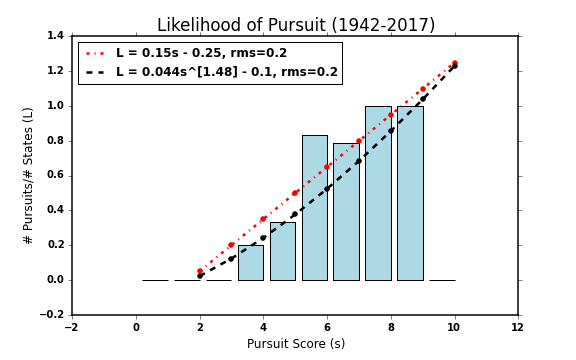
\includegraphics[scale=0.8]{./figs/pe_likely.png}
\end{center}
\caption{Fraction of states with any nuclear technology (dataset from \ref{s_factors}) that pursued weapons at some point in the last 75 years, given their pursuit scores. Although a power-law curve (black) and a weighted linear fit (red) are equivalent with the existing data, a complete set of nation-states would increase the relative weight of lower scores, making the exponential curve a better fit.}
\label{fig:likely}
\end{figure}
 
The score is then converted into a likelihood that the state will pursue a weapon. The relationship between pursuit score and likelihood of pursuing a weapon has been characterized using historical data of the 42 states that have developed nuclear technology since 1942.  \ref{fig:likely} shows the fraction of states with a given pursuit score that pursued a weapon during that time. A power-law (red) or a weighted linear fit (black) are are equivalentl with the 42 state dataset. However, a global dataset of nation-states would have disproportionately lower scores, so we consider the power-law paramaterization to be more representative.


The data shown in \ref{fig:likely} represents the total likelihood integrated over the course of 75 years ($T$). Equation \ref{eqn:likely_eqn} is used to convert to the likelihood of pursuit $L$ in any given year, given a pursuit score $s$.
\begin{equation}
L = 1 - (1 - s)^{1.0/T}
\label{eqn:likely_eqn}
\end{equation}
In the \gls{NWPM} forward model, each state's score is converted to a likelihood of pursuit at that timestep using Equation \ref{eqn:likely_eqn}. The actual conversion is bounded using two heavy-side functions such that scores below a lower threshold (e.g. 4) are forced to a likelihood of zero, while scores above an upper threshold (e.g. 9) are forced to the value of the score at the threshold.   A random number generator is used given the likelihood to determine whether or not the pursuit event occurs. If the determination is for pursuit to occur, the state deploys a secret enrichment facility. If a state is already pursuing a weapon, then the model determines whether it succeeds in acquiring a weapon at that timestep using a median time to acquire of 7.5 years, based on historical data for states that have acquired weapons. On the timestep in which a state succeeds in acquiring a weapon, highly enriched uranium is shipped out of the secret enrichment facility.

\subsection{Limitations of the Historical Data}
The use of historical data to develop a forward model has several limitations. One set of limitations could be improved with a larger historical dataset.  Historical scores for non-nuclear states have not been calculated. Due to the influence of nuclear technology, a non-nuclear state could theoretically have a maximum pursuit score of 7. Considering that the majority of states that have high potential military spending and major historical conflicts have already been incorporated, this further reduces the potential maximum score to below 5, even if all other factors were maximized.  A large fraction of states in the world are have scores on the order of 1-3.  This large set of missing historical data, heavily weighted to the low score side, would reduce the likelihood of higher-score states from pursuing.  The database could also be improved by collecting historical data for many years around dates of pursuit and acquisition rather than just for a single year. This analysis has identified factors that are correlated to weapons programs but there is insufficient data to confirm causal relationships.   

This model is intrinsically limited by the small sample size and the degree to which the global landscape changes over time. With only 10 states that have acquired nuclear weapons throughout history, there is large uncertainty in any quantatitative analysis. Additionally, while conflict has been captured in a crude way, it is difficult to develop a parameterization with enough nuance to capture the varying impact of conflict under paradigms such as World War II, the Cold War, or post-9/11.


\section{A Diversion Scenario: Highly Enriched Uranium}
\label{s_results}
As a part of the \gls{CVT}\footnote{http://cvt.engin.umich.edu/}, \Cyclus is being used to incorporate socio-behavioral modeling into simulations of \gls{HEU} diversion from a declared fuel cycle with the goal of improving multi-modal anomaly detection techniques.  In the simplest implementation, material is diverted from the enrichment facility.  Figure \ref{fig:heu_layout} illustrates a toy model of this portion of the fuel cycle. A facility such as a mine supplies natural uranium (0.7\% $^{235}$U) to an enrichment facility. 

**** Use UM analysis?: Multi-enrichment scenario cartoon, QTY/SWU for simple case, QTY/SWU for tails distribution, and resulting detection (From Yasin)











 The enrichment facility in turn receives requests for  \gls{LEU} (4\% $^{235}$U) from a declared light-water reactor (ignoring the fuel fabrication facility for simplicity).  The enrichment facility also receives requests for 90\% enriched \gls{HEU} from an undeclared actor seeking to build a nuclear weapon. Material production for each facility is calculated once each month for a total of 100 months.  This framework allows us to pose the following question: If an inspector only has access to the inventory records for the \gls{LEU} that arrives at the declared reactor, can diversion of material be detected?

\begin{figure}%[htbp!]
\begin{center}
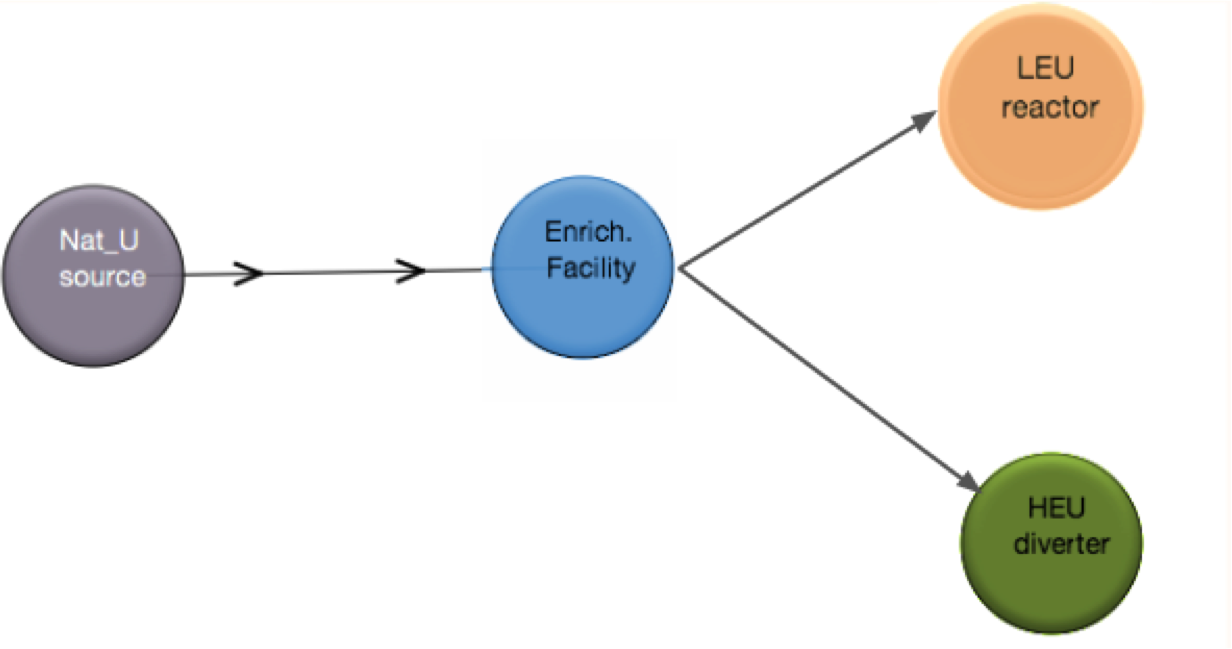
\includegraphics[natwidth=162bp,natheight=227bp, scale=0.6]{./figs/heu_cyclist_layout.png}
\end{center}
\caption{Agent layout and material flow for a toy model of \gls{HEU} diversion from a declared fuel cycle at the enrichment facility.}
\label{fig:heu_layout}
\end{figure}

To make the scenario more realistic, three conditions are applied to the simulation:
\begin{itemize}
\item{The enrichment facility is operating near its maximum \gls{SWU} limit}
\item{The demand for \gls{LEU} material has a time-varying amplitude with a Gaussian distribution}
\item{The enrichment facility will always prioritize fulfilling requests for \gls{HEU}}
\end{itemize}
The \gls{SWU} limit, a metric that incorporates power-consumption and maximum processing throughput, constrains the simulation so that if the enrichment facility chooses to produce \gls{HEU} then its \gls{LEU} output will necessarily decrease.  If the \gls{LEU} demand were constant then there would be a clear signature of diversion when \gls{HEU} was produced.  A time-variation in \gls{LEU} demand is more representative of real-life, where a single enrichment facility provides fuel to many reactors, which may operate on different reloading schedules. Variations in demand can also be caused by unanticipated reactor shutdowns, delays in receiving raw material, maintenance and repairs, etc.  While these events are somewhat mitigated in real operations by the use of long-term contracts and material reserves, a small variation in \gls{LEU} demand is a reasonable assumption.

% Simulation parameters in RS_3sink.xml at
%/Users/mbmcgarry/git/data_analysis/data/v1.2/random_sink/
\begin{table}
\centering
\begin{tabular}{|c|c|c|}
\hline
\textbf{General}    & Duration (months)       & 100  \\
\textbf{Simulation} & Natural U (\% $^{235}U$) & 0.7  \\
\textbf{Parameters} & LEU (\% $^{235}U$)       & 4.0  \\
                    & HEU (\% $^{235}U$)       & 90.0 \\
\hline
\textbf{Enrichment} & SWU Capacity (kg-SWU/month) & 180  \\
\textbf{Facility}   & Tails Assay (\% $^{235}U$)   & 0.3  \\
\hline
\textbf{LEU Demand} & Mean Qty (kg)       & 33.0  \\
                    & $\sigma$ (kg)       & 0.5  \\
\hline
\textbf{HEU Demand} & Qty (kg)            & 0.03  \\
                    & Avg Rate of Occurrence & 1/5 \\ 
\hline
\end{tabular}
\caption{Simulation parameters for \gls{HEU} diversion scenario.}
\label{tab:sim_params}
\end{table}


Several behavioral models have been explored to parameterize the behavior of the illicit actor who is requesting \gls{HEU}.   In the scenario presented here, the actor asks for the same quantity of material in each request, but the requests are not made at regular intervals. Rather they are modeled as occurring `randomly' with a Gaussian distribution that defines their average rate of occurrence.  Other models that have been examined include diversion at regular intervals, as well as independent engagement decision-making for both the illicit actor and the enrichment facility.  Table \ref{tab:sim_params} lists the parameters used for the simulation, where \gls{HEU} is diverted using the `random' model with an average occurrence rate of once per 5 months.  Figure \ref{fig:heu_demand} shows the \gls{HEU} demand from the illicit actor as a function of time.  Figure \ref{fig:leu_produced} illustrates the impact of this illicit material diversion on overall \gls{LEU} production.  The orange trace represents the amount of \gls{LEU} material that would have been produced by the enrichment facility at each timestep if there had been no material diversion for \gls{HEU} production.  The blue trace represents the amount of \gls{LEU} that was actually produced and shipped to the declared reactor during the diversion scenario.


% Figures made with ~/git/data_analysis/fourier_analysis.ipynb, and saved in
% /Users/mbmcgarry/git/data_analysis/data/v1.2/random_sink/png
\begin{figure}
\begin{center}
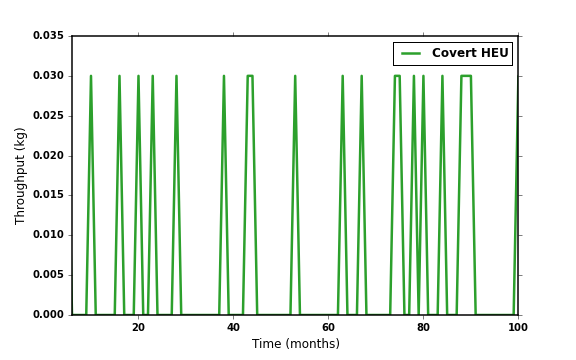
\includegraphics[natwidth=162bp,natheight=227bp, scale=0.6]{./figs/HEU_R5.png}
\end{center}
\caption{An illicit actor requests \gls{HEU} from the enrichment facility at random intervals with an average occurrence rate of 1 out of every 5 months.}
\label{fig:heu_demand}
\end{figure}

\begin{figure}
\begin{center}
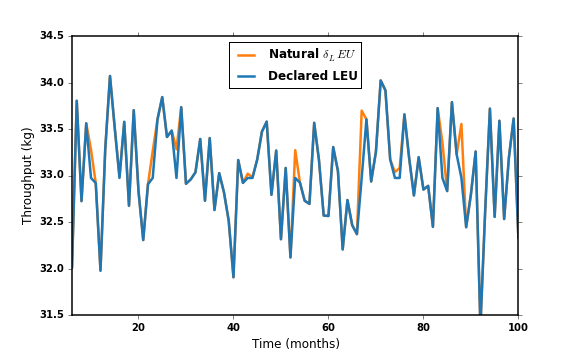
\includegraphics[natwidth=162bp,natheight=227bp, scale=0.6]{./figs/nat_delta_R5.png}
\end{center}
\caption{Expected variation of \gls{LEU} demand in the absence of diversion is shown in orange, while the \gls{LEU} actually produced in the diversion scenario is shown in blue. The amplitude of the diverted material was chosen to displace the signal with one standard deviation of the expected variation.}
\label{fig:leu_produced}
\end{figure}


\begin{figure}
\begin{center}
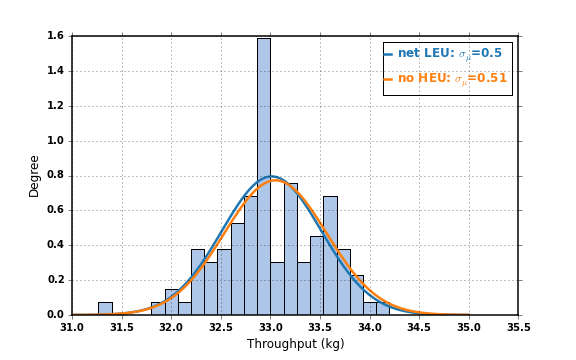
\includegraphics[natwidth=162bp,natheight=227bp, scale=0.6]{./figs/netLEU_hist_R5_new.png}
\end{center}
\caption{Distribution of LEU quantity produced in the diversion scenario (blue). The expected variation of \gls{LEU} demand in the absence of diversion is shown in orange (fitted).  A shift between the fitted curves indicates that material is being diverted.}
\label{fig:leu_histogram}
\end{figure}

If the inspector has access to only the blue time-series data, is it possible to identify whether or not material is being diverted from the system?  A naive approach is to look at the distribution of the time-series data.  Figure \ref{fig:leu_histogram} is a histogram of the declared \gls{LEU} signal showing the distribution of the quantity of \gls{LEU} that was declared.  The blue trace is a Gaussian fit to the declared data, while the orange trace (``expected'') is a Gaussian fit to the hypothetical variation in the \gls{LEU} signal if there were no diversion.  In this example, an inspector would need a sufficiently well-sampled dataset for the facility during a time when there was no diversion to characterize the expected distribution in order to draw conclusions about whether or not material diversion is occurring. An ongoing collaboration with researchers at the Michigan Institute for Data Science\footnote{http://midas.umich.edu/} seeks to apply innovative anomaly detection techniques to these simulations to investigate detection limits for scenarios with sparse data sets or low signal-to-noise ratios.





  

\section{Discussion}
\label{s_dis}

The \Cyclus fuel cycle simulator is being used as a framework for combining techniques and knowledge from a variety of disciplines into a cohesive treaty verification approach. This paper presents the diversion of \gls{HEU} as a simple example of measuring facility output as a treaty verification strategy.  This \gls{HEU} simulation used a random-interval, constant-amplitude model to describe the behavior of an illicit actor seeking to divert \gls{HEU} from a declared enrichment facility.  It uses statistical anomaly detection techniques on the data that would be available to an \gls{IAEA} inspector, namely the \gls{LEU} output of the enrichment facility, to demonstrate that material diversion could be detected in this scenario.

This simulation is but one example of the capabilities of \Cyclus as a test bed for treaty verification strategies.  \Cyclus is also being used to model the geographical dissipation of $^{85}Kr$ emission from a covert separations facility processing \gls{WGP} in the effluent shadow of declared facilities.  This feature can be used to assess the required regional distribution of various types of $^{85}Kr$ detectors to ensure detection of clandestine reprocessing programs.  Additionally, \Cyclus has the capability to produce synthetic signals of inherent physical processes such as neutron spectra of various materials.  In this way, \Cyclus simulations can provide theoretical signals to researchers developing experimental detectors in order to test sensitivity and detector response.

Moving forward, \Cyclus will be used to study more complex diversion scenarios.  Probabilistic models for behavior based on risk-perception will be explored.  Ongoing collaborations as part of the \gls{CVT} are examining the mechanisms and limits of expanding anomaly detection algorithms with other types of data, such as social media chatter.  Due to the inherently interdisciplinary nature of this work, new external collaborations are sought with experts in behavioral modeling. Innovative ideas on detection modalities and diversion detection techniques are also welcomed.



\textit{\TODO{This work is funded by the NNSA as part of the Consortium for Verification Technology.  . ..}}

%%%%%%%%%%%%%%%%%%%%%%%%%%%%%%%%%%%%%%%%%%%%%%%%%%%%%%%%%%%%%%%%%%%%%%%%%%%%%%%%
\bibliographystyle{ANSurl}
\bibliography{../zotero_150923,../websites_manual}
%\bibliography{/Users/mbmcgarry/git/papers/zotero_150918}
\end{document}
